
\chapter*{EXAME: MS680 - MT624 - II Sem 2020}
\addcontentsline{toc}{chapter}{\textcolor{blue}{PROVA 04: MS680 - MT624 - II Sem 2020}}

\begin{quote}
\textbf{POSTADA}: 21 de Janeiro de 2021 (Quinta - feira)

\textbf{RECEBIMENTO}: 25 de Janeiro de 2021 (Segunda - feira - 08:00 horas da manhã)

\textbf{ATENÇÃO}:

\begin{description}
\item 1 - As Questões devem ser encaradas como \textbf{oportunidades} para demonstrar conhecimento e não como perguntas.

\textbf{Precisão} e \textbf{Concisão} serão qualidades avaliadas. Portanto, \textbf{atente para o enunciado das questões} para evitar uma exposição de fatos e desenvolvimentos não relacionados ou não solicitados.

\item 2 - A redação de cada Exame deve apresentar a forma de um depoimento pessoal distinto.Caso ocorram semelhanças exageradas em redações de origens distintas, todos os Exames envolvidos receberão a avaliação I (Insuficiente).

\item 3 - Cada Questão resolvida deve ser precedida de seu respectivo Enunciado Original completo.

\item 4 - A Resolução deve ser \textbf{digitalizada} em um \textbf{único documento pdf} (\textit{Manuscritos} \textbf{NÃO} serão aceitos!)

\item 5 - O documento pdf da Resolução deve ser enviado no \textbf{Anexo} de uma mensagem com título ``\textbf{EXAME}'' para o endereço eletrônico: wilson@unicamp.br

\item 6 - Não deixe para resolver, redigir e/ou enviar a sua Prova na última hora e evitando assim ser responsabilizado por acidentes imprevisíveis, mas possíveis (Lei de Murphy).
\end{description}
\end{quote}



\clearpage
\chapter*{Questão 01: -Método de Fourier e Difusão Compartimental}
\addcontentsline{toc}{section}{\textcolor{blue}{Questão 01}}


Considere um Modelo Matemático descrito por funções
\[\begin{array}{rcl}
x: \mathbb{R} &\to& \mathbb{C}^n \\
t &\mapsto& x(t) = (x_1(t), x_2(t), x_3(t))^t,
\end{array}\]
definidas Newtoniamente como soluções de uma equação diferencial vetorial ``Malthusiana'' da forma \(\dfrac{dx}{dt} = Sx\), em que \(S\) é uma matriz real e simétrica:
\begin{eqnarray}\label{eq:edoprova03q01}
\dfrac{dx}{dt} =
\left(\begin{array}{c}
\dfrac{dx_1}{dt} \\[0.5cm]
\dfrac{dx_2}{dt} \\[0.5cm]
\dfrac{dx_3}{dt}
\end{array}\right) =
\left(\begin{array}{ccc}
-2 & 1 & 0 \\
1 & -2 & 1 \\
0 & 1 & -2
\end{array}\right)
\left(\begin{array}{c}
x_1 \\
x_2 \\
x_3
\end{array}\right)
= S x.
\end{eqnarray}

\begin{description}
\item[A -] Interprete, justificando, esta Equação Diferencial vetorial como Modelo para um processo de Difusão entre 3 compartimentos na forma
\[\longleftarrow\ A_1\ \substack{\ \longleftarrow \\ \longrightarrow\ }\ A_2\ \substack{\ \longleftarrow \\ \longrightarrow\ }\ A_3\ \longrightarrow\]

\item[B -] Obtenha todas as soluções básicas de Fourier para este sistema na forma \(h(t) = e^{\lambda t} v\), com \(||v|| = 1\).

\item[C -] Calcule a solução da Equação com condição inicial
\(x_1(0) = 1\), \(x_2(0) = 0\), \(x_3(0) = 0\), ou seja, \(x(0) = \left(\begin{array}{c} 2 \\ 1 \\ 3\end{array}\right)\).

\item[D -] Calcule a solução da Equação com condição inicial geral
\(x(0) = \alpha \in \mathbb{C}^3\) e mostre que \(\displaystyle\lim_{t \to \infty} x(t) = 0\), interpretando o resultado em termos do Modelo.

\item[E -] Mostre que o sistema pode ser linearizado assintoticamente na forma \(\displaystyle\lim_{t \to \infty} \dfrac{\log||x(t)||}{\lambda t} = 1\) e determine \(\lambda\).

\item[F -] Considere uma população inicial \(N_0\) toda concentrada no compartimento central, isto é, \(x_1(0) = 0\), \(x_2(0) = N_0\), \(x_3(0) = 0\). Calcule o tempo médio de \textit{permanência} destes indivíduos no sistema.
\end{description}


\clearpage

\subsection*{\blue Resolução 1 - \textbf{A}}
\addcontentsline{toc}{subsection}{\textcolor{blue}{Resolução 1 - \textbf{A}}}

Reescrevamos a equação \eqref{eq:edoprova03q01} da seguinte maneira:
\begin{eqnarray}\label{eq:edoprova03q01a}
\begin{array}{rcl}
\dfrac{dx_1}{dt} &=& -2x_1 + x_2 \\[0.5cm]
\dfrac{dx_2}{dt} &=& x_1 - 2x_2 + x_3 \\[0.5cm]
\dfrac{dx_3}{dt} &=& x_2 - 2 x_3
\end{array}
\end{eqnarray}

Neste caso, temos $3$ compartimentos adjacentes $A_1$, $A_2$ e $A_3$ com quantidade de indivíduos, respectivamente, iguais a $x_1$, $x_2$ e $x_3$. 
A troca de indivíduos entre os compartimentos é percebida pela forma apresentada na equação \eqref{eq:edoprova03q01a}. Os compartimentos $A_1$
e $A_3$ doam indivíduos para $A_2$, ao tempo que recebem de $A_2$ e ainda, perdem indivíduos para o resto do universo. Já o compartimento central $A_2$, além da referida doação de indivíduos para os compartimentos $A_1$ e $A_3$, recebe indivíduos destes.


\subsection*{\blue Resolução 1 - \textbf{B}}
\addcontentsline{toc}{subsection}{\textcolor{blue}{Resolução 1 - \textbf{B}}}


As soluções básicas de Fourier para \eqref{eq:edoprova03q01} são da forma:
\[x^k(t) = e^{\lambda_k t} v^k,\ k =1, 2, 3\]
onde \(\lambda_k\) são os autovalores de $S$ associados aos seus respectivos autovetores \(v^k\) ortonormais. 

Para determinarmos os autovalores, devemos encontrar a solução da equação:
\begin{equation}\label{eq:polinomiocaracteristicodeS}
\det(S-\lambda I) = 0,
\end{equation}
em que \(I\) é a matriz identidade de ordem \(3\).

A solução de \eqref{eq:polinomiocaracteristicodeS} é \(\lambda_1 = -2-\sqrt{2}\), \(\lambda_2 = -2\) e \(\lambda_3 = -2+\sqrt{2}\) e os respectivos autovetores são:
\[\begin{array}{rcl}
v^1 &=& \left(\begin{array}{ccc}\dfrac{1}{2} & -\dfrac{\sqrt{2}}{2} & \dfrac{1}{2} \end{array}\right)^t \\[0.5cm]
v^2 &=& \left(\begin{array}{ccc} -\dfrac{\sqrt{2}}{2} & 0 & \dfrac{\sqrt{2}}{2} \end{array}\right)^t \\[0.5cm]
v^3 &=& \left(\begin{array}{ccc}\dfrac{1}{2} & \dfrac{\sqrt{2}}{2} & \dfrac{1}{2} \end{array}\right)^t.
\end{array}\]

Portanto, as soluções básicas de Fourier são:
\(
x_1(t) = e^{(-2-\sqrt{2}) t} \left(\begin{array}{ccc}\dfrac{1}{2} & -\dfrac{\sqrt{2}}{2} & \dfrac{1}{2} \end{array}\right)^t\),
\(x_2(t) = e^{-2 t} \left(\begin{array}{ccc}-\dfrac{\sqrt{2}}{2} & 0 & \dfrac{\sqrt{2}}{2} \end{array}\right)^t\) e 
\(x_3(t) = e^{(-2+\sqrt{2}) t} \left(\begin{array}{ccc} \dfrac{1}{2} & \dfrac{\sqrt{2}}{2} & \dfrac{1}{2} \end{array}\right)^t.
\)




\subsection*{\blue Resolução 1 - \textbf{C}}
\addcontentsline{toc}{subsection}{\textcolor{blue}{Resolução 1 - \textbf{C}}}



Uma solução para a equação \eqref{eq:edoprova03q01} é dada por:
\[x(t) = \displaystyle\sum_{k=1}^{3} c_k x^k(t) = \sum_{k=1}^{3} c_k e^{\lambda_k t} v^k.
\]

Como \(x(0) = x_0 = \left(\begin{array}{ccc} 1 & 0 & 0 \end{array}\right)^t\), temos:
\[\begin{array}{rcl}
c_1 &=& (v^1)^t \cdot x_0 = \dfrac{1}{2} \\
c_2 &=& (v^2)^t \cdot x_0 = -\dfrac{\sqrt{2}}{2} \\
c_3 &=& (v^3)^t \cdot x_0 = \dfrac{1}{2}
\end{array}\]
e a solução de \eqref{eq:edoprova03q01} fica
\[
x(t) =
\dfrac{1}{2} e^{(-2-\sqrt{2}) t}
\left(\begin{array}{c}\dfrac{1}{2} \\[0.5cm] -\dfrac{\sqrt{2}}{2} \\[0.5cm] \dfrac{1}{2} \end{array}\right) 
- \dfrac{\sqrt{2}}{2} e^{-2 t}
\left(\begin{array}{c} -\dfrac{\sqrt{2}}{2} \\[0.5cm] 0 \\[0.5cm] \dfrac{\sqrt{2}}{2} \end{array}\right)
+ \dfrac{1}{2} e^{(-2+\sqrt{2}) t} 
\left(\begin{array}{c} \dfrac{1}{2} \\[0.5cm] \dfrac{\sqrt{2}}{2} \\[0.5cm] \dfrac{1}{2} \end{array}\right)
\]



\subsection*{\blue Resolução 1 - \textbf{D}}
\addcontentsline{toc}{subsection}{\textcolor{blue}{Resolução 1 - \textbf{D}}}


Considere a equação \eqref{eq:edoprova03q01} com condição inicial geral dada por \(x(0) = \alpha = \left(\begin{array}{ccc} \alpha_1 & \alpha_2 & \alpha_3 \end{array}\right)^t\).

Como sua solução é uma combinação linear da suas soluções básicas de Fourier, que são da forma \(x^k(t) = e^{\lambda_k t} v^k\), com autovalores \(\lambda_k\) e seus respectivos autovetores \(v^k\) de \(S\) e \(k = 1, 2, 3\), temos:
\[
x(t) = \displaystyle\sum_{k=1}^{3} c_k e^{\lambda_k t} v^k.
\]
Para \(t=0\), temos:
\[\alpha = \displaystyle\sum_{k=1}^{3} c_k v^k \]
e, para cada autovetor \(v^j\), \(j = 1, 2, 3\), temos:
\[
(v^j)^t \alpha = (v^j)^t \displaystyle\sum_{k=1}^{3} c_k v^k = \displaystyle\sum_{k=1}^{3} c_k (v^j)^t v^k
\]
Uma vez que, \(v^j v^k = 0\), para \(j \ne k\), e \(v^j v^k = 1\), para \(j=k\), temos:
\[c_j = (v^j)^t \alpha.\]

Como os autovalores \(\lambda_k, k = 1, 2, 3\) de \(S\) são todos negativos, \(e^{\lambda_k t} \longrightarrow 0, \forall k\), à medida que os valores de \(t\) crescem, indefinidamente. Dessa forma,
\[
\displaystyle\lim_{t \to \infty} x(t) = \displaystyle\lim_{t \to \infty} \displaystyle\sum_{k=1}^{3} c_k e^{\lambda_k t} v^k = (0 \ \ 0 \ \ 0)^t.
\]

Isso mostra que a população irá se extinguir. Já era de se esperar isto visto a dinâmica da população retratada pelo sistema de equações diferencial (já comentada no item A).




\subsection*{\blue Resolução 1 - \textbf{E}}
\addcontentsline{toc}{subsection}{\textcolor{blue}{Resolução 1 - \textbf{E}}}


Temos que
\[
||x(t)||
= \sqrt{\displaystyle\sum_{k=1}^{3} c_k^2 e^{2\lambda_k t}}
= e^{\lambda_s t} \sqrt{\displaystyle\sum_{k=1}^{3} c_k^2 e^{2(\lambda_k-\lambda_s) t}},
\]
para \(\lambda_s = \max\{\lambda_k\},\ k = 1,\ 2,\ 3\).

Sendo assim,
\[
\displaystyle\lim_{t \to \infty}
\dfrac{\log(||x(t)||)}{\lambda t}
=
\displaystyle\lim_{t \to \infty}
\dfrac{\lambda_s t + \log\left(\sqrt{\displaystyle\sum_{k=1}^{3} c_k^2 e^{2(\lambda_k-\lambda_s) t}}\right)}{\lambda t}
=
\dfrac{\lambda_s}{\lambda} + \displaystyle\lim_{t \to \infty}
\dfrac{\log\left(\sqrt{\displaystyle\sum_{k=1}^{3} c_k^2 e^{2(\lambda_k-\lambda_s) t}}\right)}{\lambda t}.
\]
Observamos que \(\left(\sqrt{\displaystyle\sum_{k=1}^{3} c_k^2 e^{2(\lambda_k-\lambda_s) t}}\right)\) é limitado, uma vez que \(\lambda_s \ge \lambda_k\), para todo \(k = 1, 2, 3\) e, neste caso, o sistema pode ser linearizado assintoticamente na forma
\[\displaystyle\lim_{t \to \infty}
\dfrac{\log(||x(t)||)}{\lambda t} = 1,\]
desde que \(\lambda = \lambda_s\).





\subsection*{\blue Resolução 1 - \textbf{F}}
\addcontentsline{toc}{subsection}{\textcolor{blue}{Resolução 1 - \textbf{F}}}

Seja $x(t) = \displaystyle\sum_{k=1}^{3} c_{k}e^{\lambda_{k}t}v^{k}$ uma solução para $\dfrac{dx}{dt} = Sx$.

Na resolução do item B, determinamos os autovalores de $S$ e os seus respectivos autovetores.

Como \(x(0) = \left(\begin{array}{ccc} 0 & N_{0} & 0 \end{array}\right)^t\), temos que:
\[\begin{array}{rclcl}
c_{1} &=& \left(\begin{array}{ccc} \dfrac{1}{2} & - \dfrac{\sqrt{2}}{2} & \dfrac{1}{2} \end{array}\right) \left(\begin{array}{ccc} 0 & N_{0} & 0 \end{array}\right)^{t} &=& - \dfrac{\sqrt{2}}{2}N_{0} \\
%%
c_{2} &=& \left(\begin{array}{ccc} - \dfrac{\sqrt{2}}{2} & 0 & \dfrac{\sqrt{2}}{2} \end{array}\right) \left(\begin{array}{ccc} 0 & N_{0} & 0 \end{array}\right)^{t} &=& 0 \\
%%
c_{3} &=& \left(\begin{array}{ccc} \dfrac{1}{2} & \dfrac{\sqrt{2}}{2} & \dfrac{1}{2} \end{array}\right) \left(\begin{array}{ccc} 0 & N_{0} & 0 \end{array}\right)^{t} &=& \dfrac{\sqrt{2}}{2}N_{0}
\end{array}\]

Segue que
\[\begin{array}{rclcl}
x(t) &=& - \dfrac{\sqrt{2}}{2}N_{0} e^{(-2 - \sqrt{2})t} \left(\begin{array}{ccc} \dfrac{1}{2} & - \dfrac{\sqrt{2}}{2} & \dfrac{1}{2} \end{array}\right)^{t} + \dfrac{\sqrt{2}}{2}N_{0} e^{(-2 + \sqrt{2})t} \left(\begin{array}{ccc} \dfrac{1}{2} & \dfrac{\sqrt{2}}{2} & \dfrac{1}{2} \end{array}\right)^{t} \\[0.5cm]
%%
&=& \left[\begin{array}{c}
- \dfrac{\sqrt{2}}{4}N_{0} e^{(-2 - \sqrt{2})t} + \dfrac{\sqrt{2}}{4}N_{0} e^{(-2 + \sqrt{2})t}  \\[0.5cm]
\dfrac{1}{2}N_{0} e^{(-2 - \sqrt{2})t} + \dfrac{1}{2}N_{0} e^{(-2 + \sqrt{2})t} \\[0.5cm]
- \dfrac{\sqrt{2}}{4}N_{0} e^{(-2 - \sqrt{2})t} + \dfrac{\sqrt{2}}{4}N_{0} e^{(-2 + \sqrt{2})t} 
\end{array}\right]
%%
 = \left[
\begin{array}{c}
\dfrac{\sqrt{2}}{4}e^{-2}N_{0}(e^{\sqrt{2}t} - e^{- \sqrt{2}t}) \\[0.5cm]
\dfrac{1}{2}e^{-2}N_{0}(e^{\sqrt{2}t} + e^{- \sqrt{2}t}) \\[0.5cm]
\dfrac{\sqrt{2}}{4}e^{-2}N_{0}(e^{\sqrt{2}t} - e^{- \sqrt{2}t}) 
\end{array}\right]
\end{array}\]

Tomando o tempo médio de permanência $\operatorname{TMP}$ como sendo
\[\operatorname{TMP} = \dfrac{1}{N_{0}} \displaystyle\int_{0}^{\infty}  \left(\begin{array}{ccc} -t & -t & -t \end{array}\right) \frac{dx}{dt}\ dt.\]



Entretanto
\[\begin{array}{rclcl}
\dfrac{dx}{dt} &=&
\left[\begin{array}{ccc}
2 & 1 & 0 \\[0.5cm]
1 & 2 & 1 \\[0.5cm]
0 & 1 & 2 
\end{array}\right]
\left[\begin{array}{c}
\dfrac{\sqrt{2}}{4}e^{-2}N_{0}(e^{\sqrt{2}t} - e^{- \sqrt{2}t}) \\[0.5cm]
\dfrac{1}{2}e^{-2}N_{0}(e^{\sqrt{2}t} + e^{- \sqrt{2}t}) \\[0.5cm]
\dfrac{\sqrt{2}}{4}e^{-2}N_{0}(e^{\sqrt{2}t} - e^{- \sqrt{2}t}) 
\end{array}\right] \\[0.5cm]
&=&
\left[\begin{array}{c}
\dfrac{\sqrt{2}}{2}e^{-2}N_{0}(e^{\sqrt{2}t} - e^{- \sqrt{2}t}) + \dfrac{1}{2}e^{-2}N_{0}(e^{\sqrt{2}t} + e^{- \sqrt{2}t})  \\[0.5cm]
\dfrac{\sqrt{2}}{2}e^{-2}N_{0}(e^{\sqrt{2}t} - e^{- \sqrt{2}t}) + e^{-2}N_{0}(e^{\sqrt{2}t} + e^{- \sqrt{2}t}) \\[0.5cm]
\dfrac{1}{2}e^{-2}N_{0}(e^{\sqrt{2}t} + e^{- \sqrt{2}t}) + \dfrac{\sqrt{2}}{2}e^{-2}N_{0}(e^{\sqrt{2}t} - e^{- \sqrt{2}t})
\end{array}\right] \\[0.5cm]
&=&
\left[\begin{array}{c}
\left( \dfrac{1}{2} + \dfrac{\sqrt{2}}{2} \right)e^{-2}N_{0}e^{\sqrt{2}t} + \left( \dfrac{1}{2} - \dfrac{\sqrt{2}}{2}\right)e^{-2}N_{0}e^{- \sqrt{2}t}) \\[0.5cm]
\left(1 + \dfrac{\sqrt{2}}{2} \right) e^{-2}N_{0}e^{\sqrt{2}t} + \left( 1 - \dfrac{\sqrt{2}}{2}\right)e^{-2}N_{0}e^{- \sqrt{2}t}) \\[0.5cm]
\left( \dfrac{1}{2} + \dfrac{\sqrt{2}}{2} \right)e^{-2}N_{0}e^{\sqrt{2}t} + \left( \dfrac{1}{2} - \dfrac{\sqrt{2}}{2}\right)e^{-2}N_{0}e^{- \sqrt{2}t})
\end{array}\right]
\end{array}\]

Segue que
\[\begin{array}{rcl}
\left(\begin{array}{ccc} -t & -t & -t \end{array}\right) \dfrac{dx}{dt}
&=& e^{-2}N_{0} \left( - 2 - \dfrac{3\sqrt{2}}{2} \right) e^{\sqrt{2}t} + e^{-2}N_{0} \left(-2 + \dfrac{3\sqrt{2}}{2} \right)e^{-\sqrt{2}t} \\[0.5cm]
%%
&=& e^{-2}N_{0} \left[ \left( - 2 - \dfrac{3\sqrt{2}}{2} \right)e^{\sqrt{2}t}t + \left( - 2 + \dfrac{3\sqrt{2}}{2} \right)e^{-\sqrt{2}t}t \right]
\end{array}\]
e então 
\[\begin{array}{rcl}
\operatorname{TMP}
&=& \dfrac{1}{N_{0}} \displaystyle\int_{0}^{\infty} e^{-2}N_{0} \left[ \left( - 2 - \dfrac{3\sqrt{2}}{2} \right)e^{\sqrt{2}t}t + \left( - 2 + \dfrac{3\sqrt{2}}{2} \right)e^{-\sqrt{2}t}t \right] dt
\\[0.5cm]
&=& e^{-2}\left[ \left( - 2 - \dfrac{3\sqrt{2}}{2} \right) \displaystyle\int_{0}^{\infty} e^{\sqrt{2}t}t dt + \left( - 2 + \dfrac{3\sqrt{2}}{2} \right) \displaystyle\int_{0}^{\infty} e^{-\sqrt{2}t}t dt. \right] 
\\[0.5cm]
&=& e^{-2}\left[ \left( - 2 - \dfrac{3\sqrt{2}}{2} \right) \dfrac{1}{(-\sqrt{2})} + \left( - 2 + \dfrac{3\sqrt{2}}{2} \right) \dfrac{1}{\sqrt{2}} \right]
\\[0.5cm]
&=& e^{-2}\left[ \dfrac{2}{\sqrt{2}} + \dfrac{3}{2} - \dfrac{2}{\sqrt{2}} + \dfrac{3}{2}  \right]
= 3e^{-2}
\end{array}\]

\textbf{Observação}: Nas integrais existentes na segunda igualdade foi utilizado o resultado: \[\displaystyle\int_{0}^{\infty} t\ e^{-\mu t}\ dt = \dfrac{1}{\mu}\] já calculado em prova anterior.


\clearpage
\chapter*{Questão 02: Médias e Homogenização}
\addcontentsline{toc}{section}{\textcolor{blue}{Questão 02}}

Interprete \(x = (x_1, \ldots, x_n) \in \mathbb{R}_+^n\) como representação de uma população subdividida em subpopulações \(x_k\).

Defina uma população descrita pela distribuição \(x\) como sendo homogênea quando (obviamente): \(x_1 = x_2 = \ldots = x_{n-1} = x_n\).

Defina uma medida de heterogeneidade para estas populações de forma ``óbvia'' como \(\mu(x) = \) ``Distância mínima entre o ponto \(x\) e a reta bissetriz \((1, \ldots, 1)\) que tem suas coordenadas iguais''.


\begin{description}
\item[A -] Obtenha o ponto da reta bissetriz que melhor aproxima \(x\) e interprete suas coordenadas em termos de uma média.
\item[B -] Obtenha uma expressão para \(\mu(x)\).
\item[C -] Interprete esta distância em termos de uma média KN.
\item[D -] Mostre que a dinâmica do sistema da questão 03 tende a homogenizar a população no sentido do limite \(\mu(x(t)) \downarrow 0\) monotonicamente quando \(t \to \infty\).
\item[E -] Interprete o resultado \textbf{D} em termos das hipóteses que fundamentam o Modelo de Difusão e argumente sobre a plausibilidade deste resultado.
\end{description}


\clearpage

Seja \(x = (x_1, \ldots, x_n) \in \mathbb{R}_+^n\) a representação de uma população em que cada \(x_k\) apresenta uma parte da quantidade de indivíduos de \(x\). Dizemos a população \(x\) é homogênea quando a distribuição de seus indivíduos é feita em partes iguais, ou seja, \(x_1 = x_2 = \ldots = x_{n-1} = x_n\).

Definamos, agora, a seguinte medida:
\begin{equation}
\mu_\xi(x) = \sqrt{\displaystyle\sum_{k=1}^{n} (x_k-\xi)^2},
\end{equation}
em que \(\mu_\xi(x)\) representa a distância a qual a população \(x\) se encontra de uma população homogênea \((\xi, \ldots, \xi) \in \mathbb{R}_+^n\). Assim, se \(\mu_\xi(x) \ne 0\), \(x\) é não homogênea e \(\mu_\xi(x)\) representará uma medida de sua heterogeneidade.




\subsection*{\blue Resolução 2 - \textbf{A}}
\addcontentsline{toc}{subsection}{\textcolor{blue}{Resolução 2 - \textbf{A}}}

Para encontrarmos um ponto da bissetriz (1, \ldots, 1) que melhor aproxima \(x = (x_1, \ldots, x_n) \in \mathbb{R}_+^n\), vamos minimizar a função:
\[
\sigma(\xi)
= [\mu_\xi(x)]^2
= \displaystyle\sum_{k=1}^n x_k^2 - 2\xi x_k + \xi^2
= \displaystyle\sum_{k=1}^n x_k^2 - 2\xi \sum_{k=1}^n x_k + \sum_{k=1}^n \xi^2
\]

Tomando \(M_A(x) = \dfrac{1}{n}\displaystyle\sum_{k=1}^n x_k\) (média aritmética) e \(M_2(x) = \sqrt{\dfrac{1}{n}\displaystyle\sum_{k=1}^n x_k^2}\) (média quadrática), podemos reescrever a última equação como:
\[
\sigma(\xi) = n \xi^2 -2n M_A(x)\xi+n [M_2(x)]^2. 
\]

Segue que
\[\dfrac{d\sigma(x)}{d\xi} = 0
\Rightarrow
2n\xi-2n M_A(x) = 0
\Rightarrow
\xi = M_A(x).
\]


\subsection*{\blue Resolução 2 - \textbf{B}}
\addcontentsline{toc}{subsection}{\textcolor{blue}{Resolução 2 - \textbf{B}}}


Podemos, nessas condições, estabelecer uma expressão para \(\mu_\xi(x)\) substituindo o valor de \(\xi\) encontrado, ou seja
\[\mu_\xi(x) = \sqrt{n\left\{[M_2(x)]^2-\left[M_A(x)\right]^2\right\}} = \mu(x).\]


\subsection*{\blue Resolução 2 - \textbf{C}}
\addcontentsline{toc}{subsection}{\textcolor{blue}{Resolução 2 - \textbf{C}}}


Se tomarmos a função identidade \(\varphi(x) = x = \varphi^{-1}(x)\), temos que:
\[M_A(x)
= \dfrac{1}{n} \displaystyle\sum_{k=1}^{n} x_k
= \dfrac{1}{n} \displaystyle\sum_{k=1}^{n} \varphi(x_k)
= \varphi^{-1} \left[\dfrac{1}{n} \displaystyle\sum_{k=1}^{n} \varphi(x_k)\right]
= M_\varphi(x)
\]

Agora, tomando a função \(\vartheta(x) = x^2\), temos \(\vartheta^{-1}(x) = \sqrt{x}\) e
\[M_2(x)
= \sqrt{\dfrac{1}{n} \displaystyle\sum_{k=1}^{n} x_k^2}
= \sqrt{\dfrac{1}{n} \displaystyle\sum_{k=1}^{n} \vartheta(x_k)}
= M_\vartheta(x)
\]

Assim, podemos reescrever a equação de \(\mu(x)\) em função das médias KN \(M_\varphi\) e \(M_\vartheta\), da seguinte maneira:
\[\mu(x) = \sqrt{n\left\{[M_\vartheta(x)]^2-\left[M_\varphi(x)\right]^2\right\}}.\]





\clearpage
\chapter*{Questão 03: Principio de Conservação unidimensional}
\addcontentsline{toc}{section}{\textcolor{blue}{Questão 03}}

Considere uma população distribuída continuamente em um espaço de aspecto unidimensional representado por \(\mathbb{R}^+\) onde é definido um ``Campo de velocidades'' v(x) que determina a taxa de modificação do aspecto x em termos dele mesmo.

\begin{description}
\item[A -] Se $x_1(t)$ e $x_2(t)$ são dois pontos móveis no espaço de aspecto que ``seguem'' o movimento determinado por $v(x)$, isto é, $\dfrac{dx_k}{dt} = v(x_k)$, com \(x_1(0) \le x_2(0)\), analise o sentido (no modelo) para a expressão
\[\dfrac{d}{dt}\left(\displaystyle\int_{x_1(t)}^{x_2(t)} \rho(x,t)\ dx\right).\]

\item[B -] \textbf{Desenvolva} a expressão acima em três expressões distintas,

\item[C -] \textbf{Interprete} as expressões matemáticas obtidas em B) em \textbf{termos do Modelo} identificando \textbf{justificadamente} o conceito de Fluxo de Transporte \(J(x,t)\).

\item[D -] Obtenha, \textbf{utilizando este artifício}, a Equação Diferencial Parcial que descreve o Modelo demográfico de Euler no espaço etário que contempla apenas uma mortalidade malthusiana heterogênea quanto à idade (sem reprodutividade).

\item[E -] Recupere o Modelo de Malthus homogêneo de mortalidade a partir do resultado obtido em \textbf{D}.
\end{description}


\clearpage

\subsection*{\blue Resolução 3 - \textbf{A}}
\addcontentsline{toc}{subsection}{\textcolor{blue}{Resolução 3 - \textbf{A}}}

Considere uma população $x$ distribuída continuamente, segundo Euler, em um espaço de aspecto unidimensional, denotado por \(\mathbb{R}^+\), no qual é definido um ``campo vetorial de velocidades'' $v(x)$. Neste espaço, consideremos dois pontos móveis, $x_1(t)$ e $x_2(t)$, que ``seguem'' o movimento determinado por $v(x)$, ou seja, $\dfrac{dx_k}{dt} = v(x_k)$, com $a = x_1(0) < x_2(0) = b$. Além disso, consideremos também a função de fluxo $\varphi (t, x)$.

Uma vez que as trajetórias dos pontos \(x_1 = \varphi(t, a)\) e \(x_2 = \varphi(t, b)\) se movimentam com o campo, pela unicidade local de solução do Problema de Cauchy, nenhum outro ponto se encontra com eles. Sendo assim, o tamanho da população $x$ no intervalo móvel \([x_1, x_2]\) se mantém constante e igual a \(\displaystyle\int_{x_1(t)}^{x_2(t)} \rho(x,t)\ dx\) e, por sua vez, sua derivada deve ser nula.


\subsection*{\blue Resolução 3 - \textbf{B}}
\addcontentsline{toc}{subsection}{\textcolor{blue}{Resolução 3 - \textbf{B}}}


Consideremos que o intervalo $[x_1, x_2]$ carregado pelo fluxo do meio contínuo. Sendo assim, 
$$
x_1(t) = \varphi(t,a) < \varphi(t,b) = x_2(t), \quad \forall\ t.
$$

A população total existente neste intervalo, em qualquer instante, é dada por:
\begin{equation}\label{eq:intquestao03}
x(t) = \displaystyle\int_{x_1(t)}^{x_2(t)} \rho(x,t)\ dx.
\end{equation}


A taxa de variação desta população que se encontra entre os pontos $x_1(t)$ e $x_2(t)$ é $\dfrac{dx}{dt}(t)$, ou seja, a derivada com respeito a $t$ da integral em \eqref{eq:intquestao03}.

Com o objetivo de determinar esta derivada e de fixar a região de integração, faremos uma mudança de variáveis onde o integrando ficará, apenas, como função de $t$. 

Para isto, consideremos a variável $\xi$ e $x(t, \xi) = x$ para obter:
$$
x(t) = \displaystyle\int_{\xi_1(t)}^{\xi_2(t)} \rho(x(\xi,t),t)\ \dfrac{\partial x}{\partial \xi}(\xi, t) d\xi.
$$

Derivando com respeito a $t$, obtemos:
\begin{eqnarray*}
\dfrac{dx}{dt} 
=
\dfrac{d}{dt} \left(\displaystyle \int_{\xi_1}^{\xi_2} \dfrac{\partial}{\partial t} (\rho\left( x(\xi,t),t \right)) \dfrac{\partial x}{\partial \xi}(\xi,t) \right)\ d \xi
=
\displaystyle \int_{\xi_1}^{\xi_2} \left[ \left( \dfrac{\partial \rho}{\partial x}\cdot \dfrac{\partial x}{\partial t} + \dfrac{\partial \rho}{\partial t} \right)\cdot \dfrac{\partial x}{\partial \xi} + \rho \cdot \dfrac{\partial^2 x}{\partial t \partial \xi} \right]\ d \xi.
\end{eqnarray*}

Como $\dfrac{\partial x}{\partial t} = v(\xi, t)$ e
$
\dfrac{\partial^2 x}{\partial t \partial \xi} = \dfrac{\partial}{\partial \xi} \left(\dfrac{\partial x}{\partial t}\right) = \dfrac{\partial}{\partial \xi} (v(\xi, t)) = \dfrac{\partial v}{\partial x}\dfrac{\partial x}{\partial \xi},
$
temos que
\begin{eqnarray}
\dfrac{dx}{dt} 
&=&
\displaystyle \int_{\xi_1}^{\xi_2} \left( \dfrac{\partial \rho}{\partial x}\cdot v(\xi, t) + \dfrac{\partial \rho}{\partial t} + \rho \cdot \dfrac{\partial v}{\partial x} \right)\dfrac{\partial x}{\partial \xi}\ d \xi \nonumber \\
&=&
\displaystyle \int_{x_1}^{x_2} \left( \dfrac{\partial \rho}{\partial t} + \dfrac{\partial \rho}{\partial x}\cdot v + \rho \cdot \dfrac{\partial v}{\partial x} \right)\ dx \nonumber \\
&=&
\displaystyle \int_{x_1}^{x_2} \left[\dfrac{\partial \rho}{\partial t} + \dfrac{\partial}{\partial x}(\rho v) \right]\ dx,  \label{integral}
\end{eqnarray}
ou seja,
$$
\dfrac{d}{dt}\left(\displaystyle\int_{x_1(t)}^{x_2(t)} \rho(x,t)\ dx \right) = \displaystyle \int_{x_1(t)}^{x_2(t)} \left[ \dfrac{\partial \rho}{\partial t} + \dfrac{\partial}{\partial x}(\rho v) \right]\ dx.
$$

Como o tamanho da população $x$ no intervalo móvel \([x_1, x_2]\) se mantém constante e, supondo que as funções $v$ e $\rho$ possuem derivadas parciais contínuas, temos, fixado $t$, que
$$
\displaystyle \int_{x_1(t)}^{x_2(t)} \left[\dfrac{\partial \rho}{\partial t} + \dfrac{\partial}{\partial x}(\rho v) \right]\ dx = 0,\ \forall\ [x_1, x_2].
$$
Assim, o integrando é uma função nula, para todo $t$ fixado, ou seja,
$$
\dfrac{\partial \rho}{\partial t} + \dfrac{\partial}{\partial x}(\rho v) = 0,
$$
isto é, não há ganho e nem perda de indivíduos na população em $[x_1, x_2]$, mas um trasporte dela. Matematicamente, este fato pode ser reescrito por meio da integral \eqref{integral}, ou seja, 
$$
\displaystyle \int_{x_1}^{x_2} \dfrac{\partial \rho}{\partial t}\ dx = - \displaystyle \int_{x_1}^{x_2} \dfrac{\partial}{\partial x}(\rho v)\ dx = \rho(x_1,t) v(x_1,t) - \rho(x_2,t) v(x_2,t). 
$$
A equação diferencial acima é denominada EDP para a conservação da população (em meio contínuo com fluxo causado pelo campo de velocidades $v(x,t)$ e densidade de massa $\rho(x,t)$).


\subsection*{\blue Resolução 3 - \textbf{C}}
\addcontentsline{toc}{subsection}{\textcolor{blue}{Resolução 3 - \textbf{C}}}


O termo $\rho(x,t) v(x,t) = \rho v$ encontrado no item anterior nos fornece a quantidade de indivíduos que passa $x$, na direção positiva, por unidade de tempo, e é chamada de \textbf{Fluxo de Transporte de indivíduos} $J(x,t)$.








\clearpage
\chapter*{Questão 04: Saturação}
\addcontentsline{toc}{section}{\textcolor{blue}{Questão 04}}

Considere a dinâmica \textbf{sem} mortalidade de uma população que apresenta reprodutividade segundo o Modelo Malthusiano: ``\textit{A taxa de reprodução per capita é constante}'', isto é,
\[\dfrac{1}{N}\dfrac{dN}{dt} = \nu,\ \nu > 0\]
(Obviamente, assumindo, segundo o próprio Malthus, um cenário ``Zen'' 4P: Paz total, sem Pragas ou catástrofes, Produção abundante de alimentos e sem Procedimentos anticoncepcionais).


\begin{description}
\item[A -] Determine a dimensão (em termos de unidades) do parâmetro \(\nu\) e \textbf{interprete-o} biologicamente e probabilisticamente.

Introduzindo um pouco mais de realidade neste cenário, tal como sugerido pelo próprio Malthus já em 1798, consideremos as seguintes condições:

\begin{enumerate}
\item Para a simples manutenção \textbf{basal} desta população é necessária a disponibilidade de alimentos a uma \textbf{taxa} \(\gamma N\) onde \(\gamma\) é a taxa de consumo \textit{per capita} mínimo de sobrevivência.
\item Os alimentos são produzidos a uma \textbf{taxa} constante \(c\), já que dependem em ultima análise da energia solar (via fotossíntese) que, em média, incide sobre a Terra em taxa constante.
\item O parâmetro \(\nu\) de reprodutibilidade per capita não é constante, mas varia proporcionalmente com a taxa excedente de alimentos, (aquela disponível além do que a população exige para a sua manutenção basal), isto é, \(\nu = r (c - \gamma N)\), \(r\) constante.
\end{enumerate}

\item[B -] Descreva um Modelo Matemático Newtoniano para a dinâmica de uma população segundo estas hipóteses.

\item[C -] Adimensionalize este Modelo, determinando a dimensão de cada um de seus parâmetros.

\item[D -] Mostre que na dinâmica deste modelo, o tamanho \(N(t) > 0\) da população converge sempre para uma constante \(K\), isto é, \(\displaystyle\lim_{t\to \infty} N(t) = K\), e determine este valor em termos dos parâmetro do problema, \(K(r, c, \gamma)\).
\end{description}

Comente biologicamente sobre este fato.


\clearpage

\subsection*{\blue Resolução 4 - \textbf{A}}
\addcontentsline{toc}{subsection}{\textcolor{blue}{Resolução 4 - \textbf{A}}}


Temos que
\[\left[\dfrac{1}{N}\dfrac{dN}{dt}\right] = [\nu].\]
Como \([N] =P\) e \([t] = T\), temos:
\[[\nu] = P^{-1} P T^{-1} = T^{-1}.\]
Assim, \(\nu^{-1}\) tem dimensão de tempo.


%Como mencionado, a expressão \(\dfrac{1}{N}\dfrac{dN}{dt} = \nu\) representa uma taxa de variação per capita.

%Assumindo que todos os indivíduos, antigos ou recém incorporados à população, possuam a mesma chance de se reproduzirem nos instantes seguintes, \(N(t)\) representa a quantidade de indivíduos dentre os \(N_0\) iniciais que ainda não se reproduziram até o instante \(t\) .

%Biologicamente \(\nu\) é a taxa de crescimento da população reprodutiva 


\subsection*{\blue Resolução 4 - \textbf{B}}
\addcontentsline{toc}{subsection}{\textcolor{blue}{Resolução 4 - \textbf{B}}}

O modelo matemático newtoniano para a dinâmica descritas pelas hipóteses 1, 2 e 3 da questão é:
\[\dfrac{1}{N} \dfrac{dN}{dt} = r (c-\gamma N).\]


Observamos que se \(N = \dfrac{c}{\gamma}\), então \(\dfrac{dN}{dt} = 0\). Isto é, o modelo nos diz que não é desejável que haja produção de mais indivíduos visto que a população já consumiria tudo o que é produzido.




\subsection*{\blue Resolução 4 - \textbf{C}}
\addcontentsline{toc}{subsection}{\textcolor{blue}{Resolução 4 - \textbf{C}}}

Vimos que \([\nu] = T^{-1} \Rightarrow [r(c-\gamma N)] = T^{-1}\). Uma vez que \(c\) é constante, temos que \([\gamma N]\) é adimensional, implicando em \([\gamma] = P^{-1}\). Como \([\nu] = T^{-1}\), temos que \([r] = T^{-1}\).


\subsection*{\blue Resolução 4 - \textbf{D}}
\addcontentsline{toc}{subsection}{\textcolor{blue}{Resolução 4 - \textbf{D}}}

Seja $N$ uma população que segue o modelo:
\[\begin{array}{rcl}
\dfrac{1}{N} \dfrac{dN}{dt} = r (c-\gamma N)
&\Rightarrow&
\dfrac{dN}{dt} = (rc) N - (r\gamma) N^2 \\[0.5cm]
&\Rightarrow&
\dfrac{dN}{dt} - (rc) N =  - (r\gamma) N^2 \\[0.5cm]
&\Rightarrow&
-N^{-2} \dfrac{dN}{dt} + (rc) N^{-1} =  (r\gamma)
\end{array}\]

Façamos \(\varphi = N^{-1} \Rightarrow \dfrac{d\varphi}{dt} = -N^{-2} \dfrac{dN}{dt}\) e substituindo na equação anterior, temos:
\[\begin{array}{rcl}
\dfrac{d\varphi}{dt} + (rc) \varphi =  r\gamma
&\Rightarrow&
e^{(rc)t} \dfrac{d\varphi}{dt} + (rc) e^{(rc)t} \varphi =  e^{(rc)t} r\gamma \\[0.5cm]
&\Rightarrow&
\dfrac{d}{dt}\left(e^{(rc)t}\varphi(t)\right) =  e^{(rc)t} r\gamma \\[0.5cm]
&\Rightarrow&
e^{(rc)t}\varphi(t) = r\gamma \displaystyle\int e^{(rc)t}\ dt \\[0.5cm]
&\Rightarrow&
e^{(rc)t}\varphi(t) = \dfrac{\gamma}{c} e^{(rc)t} + C_1 \\[0.5cm]
&\Rightarrow&
\varphi(t) = \dfrac{\gamma}{c} + C_1 e^{-(rc)t} \\[0.5cm]
&\Rightarrow&
N(t) = \dfrac{1}{\dfrac{\gamma}{c} + C_1 e^{-(rc)t}}
\end{array}\]

Tomando \(N(0) = N_0\), temos que
\[N(0) = \dfrac{1}{\dfrac{\gamma}{c} + C_1 e^{-(rc)0}}
\Rightarrow
C_1 = \dfrac{1}{N_0} - \dfrac{\gamma}{c}
\]
Assim,
\[
N(t) = \dfrac{1}{\dfrac{\gamma}{c} + \left(\dfrac{1}{N_0} - \dfrac{\gamma}{c}\right) e^{-(rc)t}}.
\]

Quando $t \to \infty$, temos que \(N(t) \to \dfrac{c}{\gamma} = K\), capacidade que a dinâmica deste modelo populacional pode suportar.

Temos que \(\dfrac{dN}{dt} = rN(c-\gamma N) = \nu > 0\). Sendo assim,
\[
\dfrac{d^2N}{dt^2}
= \dfrac{d}{dt} (rc N - \gamma r N^2)
= rc \dfrac{dN}{dt} - 2 \gamma r N \dfrac{dN}{dt}
= r(c-2\gamma N) \dfrac{dN}{dt}
\]

Como \(\dfrac{dN}{dt} > 0\) e \(r\) é uma constante não nula,
\[
\dfrac{d^2N}{dt^2} = 0
\Leftrightarrow (c-2\gamma N) = 0
\Leftrightarrow N = \dfrac{c}{2\gamma} = \dfrac{K}{2}.
\]


A seguir, temos a Figura \ref{fig:verhult} que ilustra diferentes situações dos gráficos de \(N\) para \(0 < N_0 < \dfrac{K}{2}\), \(\dfrac{K}{2} < N_0 < K\) e \(N_0 > K\).

\begin{center}
\captionof{figure}{Modelo populacional em questão}
\label{fig:verhult}
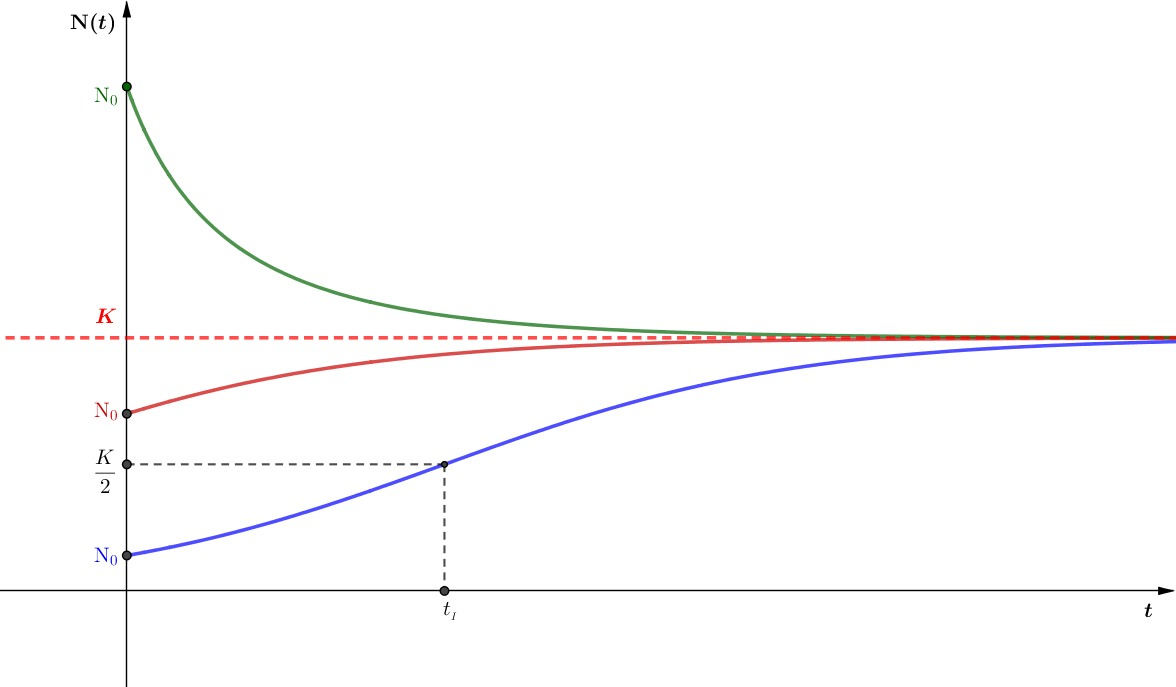
\includegraphics[height=8.cm,width=13.0cm]{figs/verhulst.jpeg}
\fonte{Figura elaborada pelo autor}
\end{center}



Quando \(0 < N_0 < \dfrac{K}{2}\), observa-se que existe um crescimento rápido da população até o tempo \(t_I = \dfrac{-1}{rc} \log\left(\dfrac{K}{N_0}-1\right)\) e depois deste, o crescimento torna-se mais lento.

Quando \(\dfrac{K}{2} < N_0 < K\), observa-se que a população apresenta, apenas, crescimento mais lento.

Quando \(N_0 > K\), observa-se que o número de indivíduos da população, para se ajustar à capacidade de suporte do meio (razão entre o que é produzido e a taxa de consumo \textit{per capita}), deve diminuir.

Em qualquer um dos casos, temos que o número de indivíduos da população tende a capacidade suporte do meio.